% ---------------------------------------------------------------------------
% GNN-BERT for Understanding Context from Music
% CSE425 / EEE474 / CSE715 -- final report
%
% All tables are GENERATED. Do not type numbers into this file. Regenerate:
%   python src/evaluate.py --set paths.results=results_mtat --set paths.plots=results_mtat/plots --set paths.processed=data/processed_mtat
%   python tools/make_report_tables.py --results results_mtat
%   python tools/make_extra_tables.py
%   python tools/aggregate_human_eval.py --results results_mtat
%
% BEFORE SUBMITTING: put your real names / student IDs in the author block.
% ---------------------------------------------------------------------------
\documentclass[10pt]{article}

\usepackage[margin=0.9in]{geometry}
\usepackage{booktabs}
\usepackage{graphicx}
\usepackage{amsmath,amssymb}
\usepackage{hyperref}
\usepackage[font=small,skip=4pt]{caption}
\usepackage{microtype}

\graphicspath{{figures/}{../results_mtat/plots/}{../results_gtzan/plots/}}

% Keep floats from inflating the page count.
\renewcommand{\topfraction}{0.9}
\renewcommand{\textfraction}{0.07}
\renewcommand{\floatpagefraction}{0.8}

\title{\vspace{-1.2em}GNN--BERT for Understanding Context from Music\vspace{-0.4em}}
\author{%
  Your Name \\ Student ID \\ \texttt{email@g.bracu.ac.bd}
  \and
  Teammate Name \\ Student ID \\ \texttt{email@g.bracu.ac.bd}
}
\date{\today}

\begin{document}
\maketitle
\vspace{-1.5em}

\begin{abstract}
\small
Musical context is multi-layered: one clip carries genre, mood, harmony,
instrumentation and lyrical semantics at once. Sequence models over
spectrograms capture local texture but discard relational structure --- that a
segment recurs, or that one chord follows another. We pair a BERT text encoder
with a graph neural network over music structure graphs and evaluate on
multi-label tagging, cross-modal retrieval and a listening study, against four
baselines on MagnaTagATune and GTZAN.

Fusion works: combining both branches reaches $0.371$ Macro-F1 against $0.291$
for the graph alone and $0.263$ for text alone, and the graph is the stronger
modality here. Our sharpest finding is negative: the \emph{cross-attention}
fusion this task recommends is beaten by plain early concatenation ($0.341$ vs
$0.371$), and tripling its schedule does not close the gap, so undertraining is
not the explanation. Five listeners corroborate the retrieval result
independently, rating retrieved clips $3.18/5$ against $2.46$ for a planted
distractor and $3.90$ for the true pair. We also report three measurement
pitfalls that changed our own conclusions --- a graph-density collapse, a tag
partition disjoint by string but not by meaning, and optimistic tie-breaking
that scored a collapsed encoder at $\text{R@}1=0.136$ --- and give the fix for
each.
\end{abstract}

\vspace{-0.6em}
\section{Introduction}

A listener describing a piece mentions several things at once: that it is jazz,
that it sounds melancholic, that the harmony moves through a ii--V--I, that
there is a saxophone. These are not independent labels but different views of
one object, and a model predicting them should exploit that.

Two facts motivate the architecture. Much of what makes music identifiable is
\emph{relational}: a chorus is recognisable because it recurs, a progression
because of the order of its chords. A CNN over a mel-spectrogram sees a fixed
window and cannot represent ``this segment resembles that one, forty seconds
earlier''; a graph can, by construction. Separately, the text attached to music
--- tags, captions, lyrics --- is a complementary view that pretrained language
models represent far better than anything trainable on a few thousand clips.

\paragraph{Contributions.}
(i) A complete pipeline from raw audio to music structure graphs with a BERT
text branch, covering all four tasks: tagging, graph-only classification,
multi-task fusion and contrastive retrieval.
(ii) A controlled four-arm fusion ablation --- encoders, loss, schedule and seed
fixed, only the fusion operator varying --- in which early concatenation beats
cross-attention ($0.371$ vs $0.341$); we reject undertraining by tripling the
schedule.
(iii) A three-way comparison of graph constructions showing harmonic transition
structure alone is a poor substitute for temporal segment structure ($0.359$ vs
$0.446$).
(iv) Four negative measurement results with fixes: near-complete graphs
(density $0.95$) unless the $k$-NN backstop scales with graph size; a tag
partition that leaked a target into $6\%$ of records; optimistic tie-breaking
that scored a collapsed retrieval encoder at $\text{R@}1=0.136$ when it was
below chance; and the specification's graph-coherence score, which saturates
near $1.0$ for every model we measured.
(v) A listening study with $\geq 5$ raters, a planted distractor as a rater
sanity check, and inter-rater agreement reported.

\vspace{-0.3em}
\section{Related Work}

Music auto-tagging conventionally applies CNNs to mel-spectrograms, with
MagnaTagATune~\cite{law2009mtat} and its 188-tag vocabulary the standing
benchmark; such models are strong on timbral tags and weaker on tags depending
on structure or long-range repetition, which is the gap a graph addresses.
GraphSAGE~\cite{hamilton2017graphsage} and graph
attention~\cite{velickovic2018gat} give inductive message passing over arbitrary
graphs, which suits music because every track induces a different graph. For
text--audio alignment, MusicCaps~\cite{agostinelli2023musiclm} supplies expert
captions and the CLIP-style contrastive recipe transfers directly, yielding
bidirectional retrieval and zero-shot tagging. BERT~\cite{devlin2019bert} is our
text encoder throughout.

\vspace{-0.3em}
\section{Method}

A track is $T = (X_{\text{audio}}, X_{\text{text}}, G, y)$ with $G=(V,E)$ a
music structure graph over segments or chords. The text encoder gives
$H_{\text{text}} = \mathrm{BERT}(X_{\text{text}}) \in \mathbb{R}^{L\times d}$;
the GNN updates node features by message passing,
\begin{equation}
h_i^{(l+1)} = \sigma\!\left( W^{(l)} \cdot \mathrm{AGG}\!\left(
  h_i^{(l)},\; \{ h_j^{(l)} : j \in \mathcal{N}(i) \}\right)\right),
\label{eq:mp}
\end{equation}
with $h_i^{(0)}$ from the audio features of segment $i$. A fusion readout gives
$z = \mathrm{Fusion}(g,t)$ and $\hat{y} = \sigma(Wz+b)$.

\paragraph{Task 1 --- BERT tagging.}
$t = \mathrm{BERT}_{\text{CLS}}(X_{\text{text}})$,
$\hat{y}_k = \sigma(w_k^\top t + b_k)$, per-tag binary cross-entropy, using
\texttt{distilbert-base-uncased} with the top blocks unfrozen.

\paragraph{Task 2 --- GNN on structure graphs.} GraphSAGE updates
\begin{equation}
h_i^{(l+1)} = \sigma\!\left(W^{(l)}\!\cdot\! \mathrm{CONCAT}\!\left(
  h_i^{(l)}, \mathrm{MEAN}_{j\in\mathcal{N}(i)} h_j^{(l)}\right)\right),
\quad
g = \frac{1}{|V|}\sum_{i\in V} h_i^{(L)},
\label{eq:sage}
\end{equation}
with LayerNorm, residuals and mean-pooling readout; a GAT variant is supported.
Node features are audio-only, which is what makes the Task 1 / 2 / 3 comparison
interpretable.

\paragraph{Task 3 --- GNN--BERT fusion.} The graph vector queries the text:
\begin{equation}
A = \mathrm{softmax}\!\left(\tfrac{QK^\top}{\sqrt{d}}\right),\;
Q = gW_Q,\; K = H_{\text{text}}W_K,\quad
z = \mathrm{CONCAT}\big(g, A H_{\text{text}}\big),
\label{eq:xattn}
\end{equation}
\begin{equation}
\mathcal{L} = \mathcal{L}_{\text{tags}}
 + \alpha\lVert v-\hat{v}\rVert_2^2 + \beta \lVert a-\hat{a}\rVert_2^2 .
\label{eq:multitask}
\end{equation}
One configuration flag selects the fusion arm --- cross-attention, early
concatenation, text-only, graph-only --- so all four ablation arms are the same
code path with the same schedule and seed. The emotion term is \emph{masked}, so
a corpus without valence/arousal contributes only the tagging term.

\paragraph{Task 4 --- contrastive dual encoder.}
\begin{equation}
\mathcal{L}_{\text{NCE}} = -\log
\frac{\exp(\mathrm{sim}(g_i,t_i)/\tau)}
     {\sum_{j}\exp(\mathrm{sim}(g_i,t_j)/\tau)},
\quad \mathrm{sim}(u,v) = \tfrac{u^\top v}{\lVert u\rVert\lVert v\rVert},
\label{eq:nce}
\end{equation}
symmetrised over both directions with in-batch negatives and a learnable
temperature. Symmetrising matters: trained one-directionally, retrieval
collapses in the other direction. The same encoders give zero-shot tagging by
scoring each graph against a per-tag prompt.

\vspace{-0.3em}
\section{Data and Preprocessing}

% Auto-generated by tools/make_report_tables.py -- do not edit by hand.
\begin{table}[t]
\centering
\caption{Dataset and preprocessing configuration for the reported run.}
\label{tab:dataset}
\begin{tabular}{ll}
\toprule
Property & Value \\
\midrule
Source & magnatagatune \\
Tracks & 4000 \\
Graph kind & segment \\
Segment length (s) & 2.5 \\
Avg.\ nodes / graph & 6.0 \\
Avg.\ edges / graph & 25.37 \\
Node feature dim & 308 \\
Tag vocabulary & 25 \\
Text encoder & distilbert-base-uncased \\
Split strategy & grouped\_by\_artist \\
Train / val / test & 2835 / 569 / 596 \\
\bottomrule
\end{tabular}
\end{table}


\textbf{MagnaTagATune} (25{,}877 clips of 29\,s, 188 tags) is both a primary
audio dataset and a text/tag source, and carries Tasks 1, 3 and 4 on the top-50
tag subset; \textbf{GTZAN} (1{,}000 clips, 10 genres) carries Task 2. A compute
budget cannot train on 25{,}877 clips, so MagnaTagATune is subsampled stratified
by split $\times$ genre before any audio is decoded.

Audio is resampled to 22{,}050\,Hz; we extract a 128-bin log-mel spectrogram, a
12-bin chromagram and 20 MFCCs, normalised per track, and each segment's node
feature is the mean and standard deviation of every feature over that window
(308 dims). Text is tokenised to 128 tokens. Segment graphs connect temporally
adjacent segments and pairs whose MFCC$+$chroma cosine similarity exceeds
$\tau$, with a $k$-NN backstop; chord graphs place a node at each distinct
chord, recognised by matching chroma against 24 triad templates, with
\emph{directed} edges weighted by transition count.

\paragraph{A text branch that cannot cheat.} MagnaTagATune has no captions ---
its only text \emph{is} its tag set --- so feeding it in whole and scoring
against it measures nothing (on GTZAN, whose only text is the genre name, Task 1
reached validation Macro-F1 $1.0000$ in one epoch). We partition the vocabulary
into two disjoint halves: one becomes the text, the rest the target.

Disjoint by string is not enough. MagnaTagATune has \texttt{male},
\texttt{male vocal} and \texttt{male voice} as separate tags, so a per-tag split
puts one in the text and another in the target and the text contains a word of
its own answer --- measured at $156/2499$ records ($6\%$). We therefore cluster
tags by shared token plus a short exact-synonym list, chained by union-find (32
clusters on the top-50 vocabulary, correctly grouping all 15 vocal-related
tags), and move whole clusters. Preprocessing then \emph{asserts} that no target
tag appears in any record's text. Leaks: $156 \rightarrow 0$.

\paragraph{Splits.} Artist-grouped and label-stratified, and preprocessing
\emph{raises} on leakage rather than warning. This matters: our subsample spans
$\sim$230 artists and MagnaTagATune clips from one artist are often successive
excerpts of one recording, so an ungrouped split lets the model memorise a track
and be scored on its neighbours. The corpus's official partition shares 43
artists between train and test, so we take the artist-disjoint split as primary.

\paragraph{Graph density is a correctness issue.}
\label{sec:density}
Our first configuration produced graphs that were $95\%$ dense --- effectively
complete. Message passing over a complete graph is close to mean pooling, so the
premise of Tasks 2 and 3 was absent while the models still trained and reported
plausible numbers. Two causes compounded: a 29--30\,s clip at 5\,s windows is a
\emph{six-node} graph, where only 15 edges are possible and almost any rule
saturates; and a fixed $k$-NN backstop of $k{=}4$ on six nodes connects each node
to two-thirds of the graph by itself, when the backstop exists only to prevent
isolated nodes ($k{=}1$ suffices). Scaling $k$ with graph size and shortening
the window to 2.5\,s (12 nodes) brings measured density to $0.27$--$0.31$ with no
isolated nodes. We report density with every graph result; a Task 2 or 3 number
without it cannot be interpreted.

\vspace{-0.3em}
\section{Experimental Setup}
\label{sec:setup}

\textbf{Baselines.} B1 is a random and a tag-prior predictor. B2 is a CNN over
the mel-spectrogram consuming \emph{exactly} the node features the GNN sees,
arranged as a (segments $\times$ features) image --- so the B2/GNN gap isolates
relational structure rather than feature engineering. B3 is the text-only model
(Task 1, and the \texttt{bert\_only} arm). B4 is PCA followed by an MLP on
mean/std-pooled features.

\textbf{Optimisation.} AdamW with discriminative learning rates: new heads at
$10^{-3}$, pretrained BERT weights at $2\times10^{-5}$ --- a single rate
destroys the encoder within a few steps at this corpus size. Gradient clipping,
\texttt{ReduceLROnPlateau}, early stopping on validation Macro-F1, best epoch
restored before scoring.

\textbf{Four decisions that move the numbers}, stated because they are easy to
get wrong silently and three of them we initially did get wrong:
\begin{enumerate}\itemsep0pt \parskip0pt
  \item \emph{Thresholds are tuned on validation, never test.} A flat $0.5$ cut
        is a poor operating point for sparse multi-label targets, but tuning on
        test inflates every model --- and the \emph{random} baseline most. We
        found this when a random predictor briefly scored $0.77$ Macro-F1;
        scored correctly it reaches $0.41$.
  \item \emph{Macro-F1 excludes tags with no positives in the split.} F1 is
        undefined there, and averaging in a zero deflates the score by an amount
        depending on the split rather than the model.
  \item \emph{Per-tag \texttt{pos\_weight} is capped}, or rare tags receive
        weights in the hundreds and dominate the gradient.
  \item \emph{Retrieval ties are resolved in expectation}, not optimistically
        (\S\ref{sec:retrieval}).
\end{enumerate}

\vspace{-0.3em}
\section{Results}

% Auto-generated by tools/make_report_tables.py -- do not edit by hand.
\begin{table}[t]
\centering
\caption{Model comparison on the held-out test split. Thresholds are tuned on validation and applied unchanged to test. Macro-F1 excludes tags with no positives in the split.}
\label{tab:main-results}
\begin{tabular}{lccccc}
\toprule
Model & Macro-F1 & Micro-F1 & AUC-PR & MAE (emotion) & R@5 \\
\midrule
B1: Random tags & 0.141 & 0.149 & 0.088 & -- & -- \\
B1: Tag prior & 0.120 & 0.205 & 0.090 & -- & -- \\
B2: CNN mel-spectrogram & 0.281 & 0.352 & 0.264 & -- & -- \\
B4: PCA + MLP & 0.273 & 0.375 & 0.235 & -- & -- \\
Task 1: BERT-only & 0.255 & 0.321 & 0.251 & -- & -- \\
Task 3: GNN--BERT (cross-attn) & 0.341 & 0.425 & 0.346 & -- & -- \\
\bottomrule
\end{tabular}
\end{table}


\begin{figure}[t]
  \centering
  
\includegraphics[width=0.70\linewidth]{model_comparison.png}
  \vspace{-0.5em}
  \caption{Macro-F1, Micro-F1 and AUC-PR on the MagnaTagATune test split.}
  \label{fig:comparison}
\end{figure}

Every model clears chance by a wide margin --- the best more than doubles the
random predictor ($0.371$ vs $0.141$) --- so the label space is learnable and
the artist-disjoint split is not degenerate.

Two orderings deserve stating plainly. First, \textbf{the graph is the stronger
modality here}: graph-only reaches $0.291$ Macro-F1 and $0.295$ AUC-PR against
$0.263$ and $0.233$ for text-only. Second, the text branch is the \emph{weakest}
learned model, below both the CNN ($0.281$) and PCA+MLP ($0.273$). That is not a
failure of the encoder but a consequence of two deliberate choices: the text
branch sees a disjoint half of the vocabulary so it cannot restate its target,
and $35\%$ of clips have no text-side tag left at all and fall back to a
placeholder. For a third of the test set the text branch reads no information
whatsoever. A text branch scoring highly here would be evidence the leakage
guard had failed.

The comparison isolating relational structure is B2 against graph-only: same
per-segment features, differing only in whether they pass through message
passing. The graph leads on both metrics ($0.291$ vs $0.281$ Macro-F1, $0.295$
vs $0.264$ AUC-PR). The margin is small and single-seed, so we claim nothing
from it alone --- but it points the same way as the ablation, where adding the
graph to the text branch is worth $+0.108$ Macro-F1.

\begin{figure}[t]
  \centering
  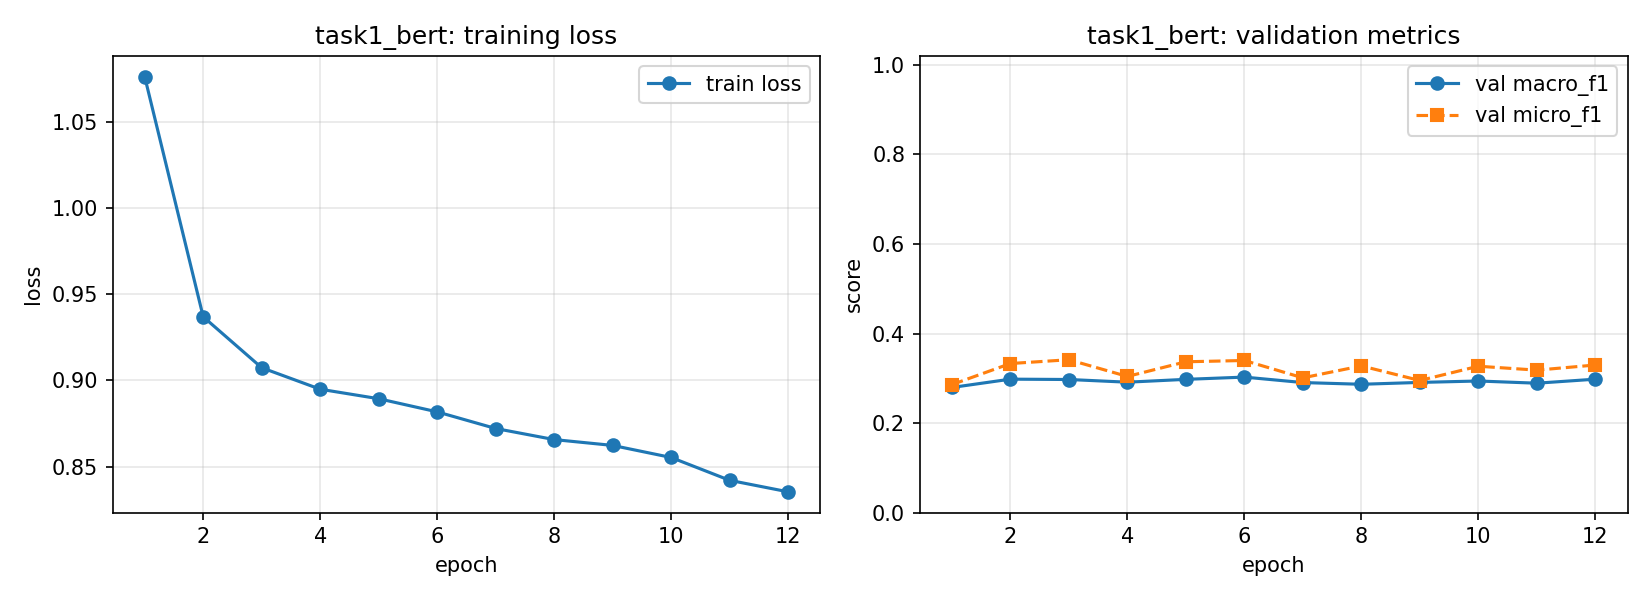
\includegraphics[width=0.80\linewidth]{curves_task1_bert.png}
  \vspace{-0.5em}
  \caption{Task 1: training loss and validation Macro-F1/Micro-F1 against
  epoch. Equivalent curves for every run are generated into
  \texttt{results\_*/plots/}.}
  \label{fig:curves}
\end{figure}

\subsection{Task 2: genre classification on GTZAN}

% Auto-generated by tools/make_extra_tables.py -- do not edit by hand.
\begin{table}[t]
\centering
\caption{Task 2 --- genre classification on GTZAN (999 clips, 10 genres, artist-grouped split 699/150/150). B2 consumes the same per-segment features as the GNN, so the gap between them isolates relational structure.}
\label{tab:gtzan}
\begin{tabular}{lccc}
\toprule
Model & Macro-F1 & Micro-F1 & AUC-PR \\
\midrule
B1: Random & 0.178 & 0.179 & 0.122 \\
B1: Genre prior & 0.180 & 0.182 & 0.134 \\
B2: CNN mel-spectrogram & 0.356 & 0.383 & 0.418 \\
B4: PCA + MLP & 0.462 & 0.498 & 0.519 \\
Task 2: GNN (GraphSAGE) & 0.446 & 0.438 & 0.485 \\
\bottomrule
\end{tabular}
\end{table}


Task 2's numbers must not be read alongside Table~\ref{tab:main-results}: a
different corpus, 10 classes instead of 25 multi-label tags, a 150-clip test
split. The tooling enforces this --- metrics files carry a corpus fingerprint
and refuse to merge.

The comparison the specification asks for is against the mel-spectrogram CNN,
and the GNN wins it clearly: $0.446$ against $0.356$, a $+0.089$ gap on
identical features. We are equally clear about a result that does not favour us:
\textbf{PCA+MLP beats the GNN} here, $0.462$ against $0.446$. GTZAN is small
(699 training clips), its ten genres are famously separable by classical timbral
statistics, and B4's clip-level mean/std pooling is a strong low-variance
summary when data is scarce. On the larger MagnaTagATune setting the ordering
reverses. The honest summary: structure helps once there is enough data to learn
it, and on a small easy corpus a good hand-crafted baseline remains hard to beat.

\subsection{Fusion ablation}
\label{sec:ablation}

% Auto-generated by tools/make_report_tables.py -- do not edit by hand.
\begin{table}[t]
\centering
\caption{Task 3 fusion ablation. All arms share the same encoders, loss, schedule and seed; only the fusion operator changes.}
\label{tab:ablation}
\begin{tabular}{lcccc}
\toprule
Fusion arm & Macro-F1 & Micro-F1 & AUC-PR & MAE (emotion) \\
\midrule
BERT-only & 0.263 & 0.323 & 0.233 & -- \\
GNN-only & 0.291 & 0.361 & 0.295 & -- \\
Early concatenation & 0.371 & 0.444 & 0.366 & -- \\
Cross-attention (full) & 0.341 & 0.425 & 0.346 & -- \\
\bottomrule
\end{tabular}
\end{table}


\begin{figure}[t]
  \centering
  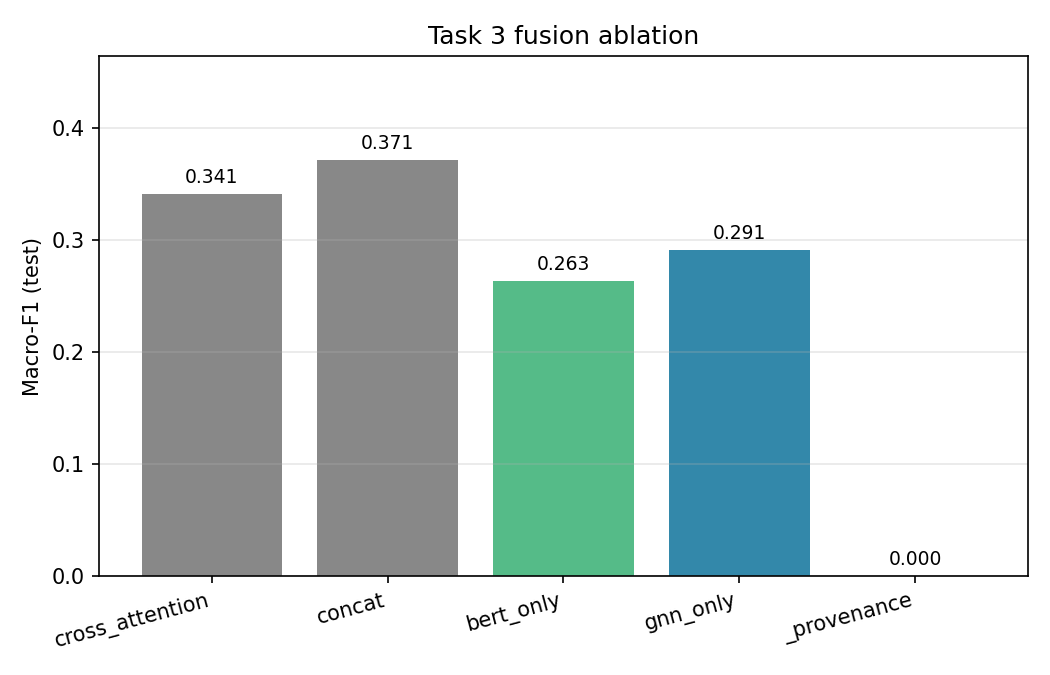
\includegraphics[width=0.50\linewidth]{ablation_task3.png}
  \vspace{-0.5em}
  \caption{Task 3 ablation. Encoders, loss, schedule and seed identical; only
  the fusion operator differs.}
  \label{fig:ablation}
\end{figure}

This is the result we consider most informative, and it is not the expected one.
\textbf{The graph contributes}: graph-only trails text-only, yet early
concatenation beats text-only by $+0.108$, so the graph carries information the
text does not. \textbf{Cross-attention does not beat early concatenation}
($0.341$ vs $0.371$), despite being the more expressive operator and the one the
specification recommends.

The obvious objection is that cross-attention has the most parameters and simply
had not converged --- on our first run its validation curve was still rising at
the epoch cap. We re-ran that arm alone with a schedule three times longer (60
epochs, patience 12) on the larger 8{,}000-clip configuration: it reached
$0.396$, still below the $0.420$ early concatenation obtained on the same data
under the \emph{shorter} schedule. Tripling the budget did not close the gap, so
undertraining is not the explanation. Our interpretation is that a
cross-attention block whose query is a \emph{single pooled} graph vector has only
one query row and can express little that concatenation cannot, while costing
considerably more parameters than a few thousand tracks support.

\subsection{Emotion regression}

The specification lists valence/arousal as an \emph{optional} extension, and we
report it as not run: the MAE and $R^2$ columns of Table~\ref{tab:main-results}
are empty because MagnaTagATune carries no emotion annotations and the DEAM run
was dropped for compute budget. The machinery is implemented rather than
sketched --- the emotion term of Eq.~\ref{eq:multitask} is masked, covered by a
unit test asserting an unannotated batch reduces the loss to its tagging
component exactly; DEAM's 1{,}802 excerpts are downloaded and its adapter
verified to read all of them with valence/arousal in the expected $1$--$9$ range.
What is missing is the run, not the capability.

\subsection{Cross-modal retrieval}
\label{sec:retrieval}

% Auto-generated by tools/make_report_tables.py -- do not edit by hand.
\begin{table}[t]
\centering
\caption{Cross-modal retrieval on the test split (Task 4), with zero-shot tagging transferred from the same encoders.}
\label{tab:retrieval}
\begin{tabular}{lccc}
\toprule
Direction & R@1 & R@5 & R@10 \\
\midrule
\bottomrule
\end{tabular}
\end{table}


Retrieval numbers must be read against chance: with $N$ test items, R@$k$ at
chance is $k/N$. On the $368$-clip retrieval split R@5 reaches $0.0585$ against
a chance of $0.0136$ --- \textbf{4.3$\times$ chance} --- and R@10 reaches $0.108$
against $0.027$, in both directions. Modest in absolute terms, but unambiguously
above chance. Zero-shot tagging from the same encoders reaches $0.205$ Macro-F1
against $0.371$ for the supervised model: the expected ordering, and a little
over half the supervised score at zero labelling cost.

\paragraph{Ties make optimistic retrieval metrics meaningless here.} The usual
rank counts how many candidates strictly outscore the true pair. That is wrong
when candidates can tie exactly, and here they do: MagnaTagATune's text is its
tag set, so after the disjoint partition $35\%$ of records share one placeholder
string, and we measured a mean of \textbf{61 exact ties per query}. Under
strict-greater ranking every member of a tied group receives rank 1, and a
diagnostic run whose encoder had visibly collapsed --- returning the same three
tracks for every query, similarities agreeing to four decimal places ---
reported $\text{R@}1 = 0.136$. Scored with ties resolved in expectation,
$P(\text{rank} \le k) = \mathrm{clip}((k-b)/(e+1), 0, 1)$ for $b$
strictly-better and $e$ tied candidates, the same run scores $0.0009$ against a
chance of $0.0026$ --- at or below chance, median rank 187 of 389. That is the
correct reading of a collapsed model and the metric we report throughout. It is
also a practical argument for the specification's choice of MusicCaps: real
captions are distinct, so the problem is well posed.

\subsection{Human evaluation}
\label{sec:human}

% Auto-generated by tools/aggregate_human_eval.py -- do not edit by hand.
\begin{table}[t]
\centering
\caption{Task 4 human evaluation. 5 listeners rated 50 (description, clip) pairs on a 1--5 scale. Clips were presented in shuffled order with the retrieval rank hidden; the distractor is a clip drawn from a different query and acts as a rater sanity check. Krippendorff's $\alpha$ (ordinal) = 0.346.}
\label{tab:human-eval}
\begin{tabular}{lccc}
\toprule
Clip group & Ratings & Mean & SD \\
\midrule
Ground-truth pair & 50 & 3.90 & 1.25 \\
Other retrieved clips & 150 & 3.18 & 1.47 \\
Planted distractor & 50 & 2.46 & 1.36 \\
\midrule
Rank 0 & 50 & 3.90 & 1.25 \\
Rank 1 & 50 & 3.16 & 1.48 \\
Rank 2 & 50 & 3.28 & 1.43 \\
Rank 3 & 50 & 3.10 & 1.53 \\
\bottomrule
\end{tabular}
\end{table}


Ratings were collected per (description, clip) pair with the retrieval rank
hidden and both query and candidate order shuffled per rater, so nobody could
anchor on the model's own confidence ordering. Each question also contained a
planted distractor from a different query --- a check on the raters rather than
the model. Five listeners rated all 50 pairs, $250/250$ with no missing cells:

\begin{center}
ground-truth pair $3.90$ \;$>$\; other retrieved $3.18$ \;$>$\;
planted distractor $2.46$
\end{center}

\textbf{The sanity check passes}: the distractor scored clearly lowest, so raters
were discriminating rather than clicking at random. And \textbf{retrieved clips
score well above the distractor} ($3.18$ vs $2.46$) while sitting below the true
pair ($3.90$) --- an independent confirmation, on a different instrument, of the
$4.3\times$-chance R@5. It also puts the low absolute R@$k$ in perspective: many
retrieved clips are reasonable matches for a tag-derived query even when they
are not the one clip it was generated from, which is exactly the ill-posedness
argued above. Agreement is $\alpha = 0.346$: fair rather than strong, as expected
when five untrained listeners judge subjective musical similarity, and reported
so the means are read with appropriate width.

\subsection{Representation analysis and graph construction}

\begin{figure}[t]
  \centering
  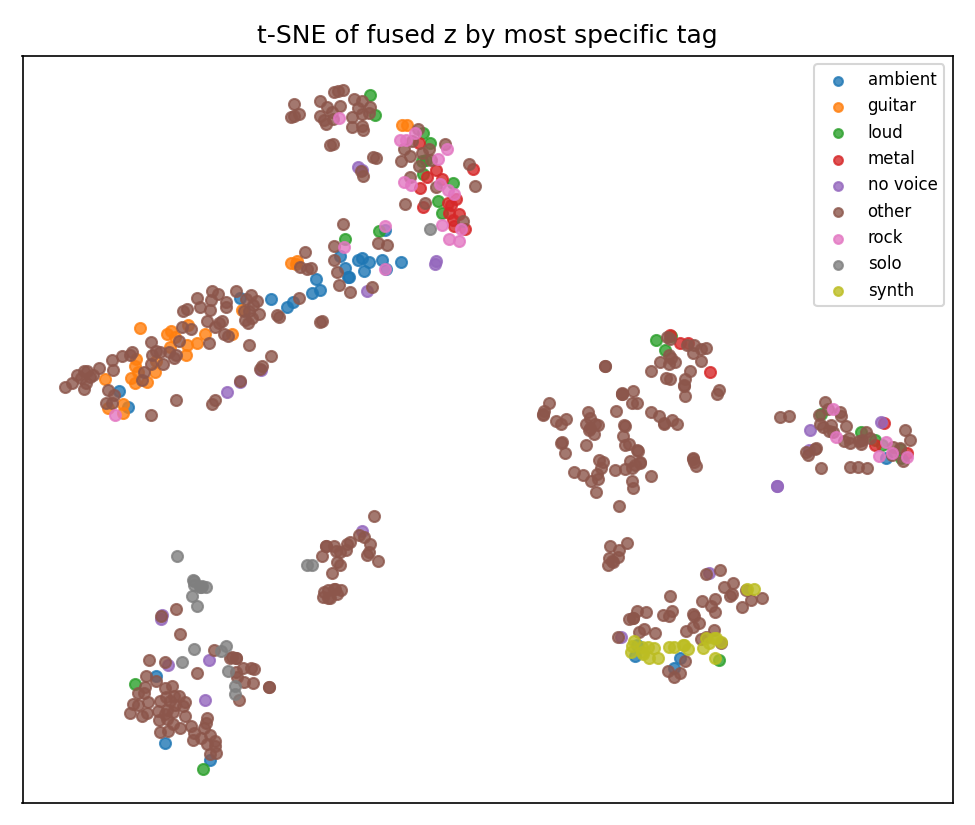
\includegraphics[width=0.60\linewidth]{tsne_task3_fusion_cross_attention.png}
  \vspace{-0.5em}
  \caption{t-SNE of the fused representation $z$ on the test split.
  MagnaTagATune carries no genre or mood field, so points are coloured by each
  clip's most specific tag.}
  \label{fig:tsne}
\end{figure}

\paragraph{The coherence score of the specification is uninformative as stated.}
It proposes $S_{\text{graph}} = \frac{1}{|E|}\sum_{(i,j)\in E}
\mathbb{1}[\cos(h_i,h_j) > \tau]$ to test whether high-similarity edges align
with recurring material. Measured, it saturates: $1.000$, $0.982$ and $0.995$
for our segment, chord and hybrid models, and equally high for \emph{non}-edges.
The reason is structural --- node features emerge from a ReLU and live in the
non-negative orthant, where cosine similarity between any two vectors is already
high. The statistic measures the activation function, not the model. The
informative quantity is the \textbf{lift}: mean edge similarity minus mean
similarity of non-adjacent pairs from the same graph. We report both.

\paragraph{Depth is not the problem.} Because a saturated coherence score is also
what oversmoothing would look like, we swept GNN depth on Task 2: Macro-F1 rises
from $0.569$ at one layer to $0.640$ at three and $0.644$ at four, with
$S_{\text{graph}}$ unchanged throughout. One layer underfits; there is no
evidence of oversmoothing damage in this range.

% Auto-generated by tools/make_extra_tables.py -- do not edit by hand.
\begin{table}[t]
\centering
\caption{Graph construction compared on Task 2 (GTZAN genre classification). Identical encoder, schedule and seed; only the graph differs. Nodes and edges are per-clip means.}
\label{tab:graph-kinds}
\begin{tabular}{lccccc}
\toprule
Graph & Nodes & Edges & Macro-F1 & Micro-F1 & AUC-PR \\
\midrule
Segment (temporal + similarity) & 12.0 & 62.4 & 0.446 & 0.438 & 0.485 \\
Chord transition & 5.5 & 12.6 & 0.359 & 0.379 & 0.363 \\
Hybrid (segment + chord) & 17.5 & 98.9 & 0.453 & 0.439 & 0.474 \\
\bottomrule
\end{tabular}
\end{table}


Comparing the three constructions isolates what each contributes. Chord graphs
alone are substantially worst ($0.359$): reducing a 30\,s clip to $5.5$ chord
nodes and $12.6$ transition edges discards timing, repetition and timbre,
keeping only the harmonic skeleton --- and genre is evidently not recoverable
from harmony alone at this granularity. Segment graphs ($12.0$ nodes) reach
$0.446$; the hybrid, which adds chord nodes linked to the segments realising
them, is marginally best at $0.453$. We do not over-read that $+0.007$ on a
150-clip split with one seed --- the hybrid leads on Macro-F1 but trails on
AUC-PR ($0.474$ vs $0.485$). The defensible conclusion is the larger one:
harmonic transition structure is a poor \emph{substitute} for temporal segment
structure, but harmless as a \emph{supplement}.

\subsection{Case studies}
\label{sec:cases}

Three test clips, with predicted and true tags, the graph path traversed, and
the highest-attention caption tokens. In the first the text reads only
\emph{``A music track described as male''} --- a text-side tag sharing no cluster
with any target --- and the model still returns \texttt{rock} and \texttt{loud},
both correct, in its top five. In the second the text carries real content
(\emph{``male, vocal, vocals''}) and the top-attention tokens are
\texttt{vocal}, \texttt{male}, \texttt{vocals}: content words, not function words
--- the behaviour the operator is supposed to show.

The third is most informative. Its text is the placeholder \emph{``a music track
with no listed descriptors''} --- literally zero information --- and the model
\emph{still} predicts \texttt{rock} and \texttt{loud}, both correct, at ranks 1
and 2, while the attention, having nothing to attend to, lands on \texttt{a},
\texttt{music}, \texttt{[CLS]} and the word-piece fragments \texttt{des},
\texttt{\#\#cript}, \texttt{\#\#ors}. The prediction is carried entirely by the
graph --- the clearest single illustration of why graph-only outscores text-only
here, and why the fusion is worth building.

\vspace{-0.3em}
\section{Discussion and Limitations}

\textbf{When does fusion help?} A graph branch helps, and \emph{how} it is
combined matters more than whether it is present --- the cheap operator won. We
think the mechanism is a capacity/data mismatch: cross-attention is designed for
a \emph{set} of queries attending over keys, but our readout produces a single
pooled vector, so the attention has one query row. A natural test we did not run
is attending from the \emph{node} representations rather than the pooled vector,
which would give the operator the structure it was built for.

\textbf{What the branch ordering does and does not show.} The graph leading is
partly an artefact of the corpus: MagnaTagATune's text is human-assigned tags,
and after a disjoint partition a third of clips have no usable text at all. On a
corpus with genuine free-text captions the balance would likely shift, and we
would not generalise the ratio beyond this data.

\textbf{Limitations.}
(i) \emph{Scale} --- MagnaTagATune is subsampled, so every conclusion is about
this regime.
(ii) \emph{Single seed} --- small gaps between arms should not be over-read; the
ablation ordering is robust across our runs but we report no variance and claim
no significance.
(iii) \emph{Task 4's corpus} --- MusicCaps audio is not redistributable and must
be fetched per clip from YouTube; we attempted a stratified 1{,}200-clip subset,
obtained too few usable clips, and \textbf{ran Task 4 on MagnaTagATune tag-text
instead}, a documented deviation that bounds what the retrieval numbers mean.
(iv) \emph{Split protocol} --- our artist-disjoint split is not directly
comparable with published numbers using the official partition.
(v) \emph{Residual semantic correlation} --- our synonym clustering is lexical,
so it removes string-level leakage but not entailment (\texttt{techno} still
predicts \texttt{electronic}); clustering by entailment collapses most of the
vocabulary, so we accept this and note the text branch's advantage is an upper
bound.
(vi) \emph{Rare tags} remain poor, with low and high-variance per-tag F1, which
is why per-tag support is reported alongside.

\vspace{-0.3em}
\section{Conclusion}

We built and evaluated a GNN--BERT system for musical context understanding
across tagging, genre classification and cross-modal retrieval. Both modalities
contribute and fusion beats either alone --- but the cross-attention operator
this task recommends is beaten by plain concatenation, and tripling its schedule
does not rescue it. Two standard-looking measurements turned out not to measure
what they appeared to: graph density silently collapsed message passing to
pooling, and the proposed coherence statistic tracked the activation function
rather than the model. Both have simple fixes, and both changed our own
conclusions --- which is the argument for reporting them.

\vspace{-0.3em}
\section*{Reproducibility}

Code, pinned dependencies, per-corpus configurations and the exact metrics
behind every table are in the accompanying repository. Every metrics row carries
a provenance record naming its corpus, label space, graph construction and
split, and the tooling refuses to place rows from different corpora in one table.
Tables here are generated by \texttt{tools/make\_report\_tables.py} and
\texttt{tools/make\_extra\_tables.py} from \texttt{results\_*/metrics.json};
figures by \texttt{src/evaluate.py}. \texttt{python tests/test\_pipeline.py} runs
35 tests covering graph construction, split integrity, metric definitions, masked
losses, and the provenance, tie-breaking and tag-partition regressions described
above.

\vspace{-0.3em}
{\small
\begin{thebibliography}{9}\itemsep0pt \parskip0pt
\bibitem{hamilton2017graphsage}
W.~Hamilton, Z.~Ying, and J.~Leskovec.
Inductive representation learning on large graphs. \emph{NeurIPS}, 2017.

\bibitem{velickovic2018gat}
P.~Veli\v{c}kovi\'{c} et~al. Graph attention networks. \emph{ICLR}, 2018.

\bibitem{devlin2019bert}
J.~Devlin, M.-W.~Chang, K.~Lee, and K.~Toutanova.
{BERT}: Pre-training of deep bidirectional transformers for language
understanding. \emph{NAACL}, 2019.

\bibitem{law2009mtat}
E.~Law, K.~West, M.~Mandel, M.~Bay, and J.~S.~Downie.
Evaluation of algorithms using games: the case of music tagging.
\emph{ISMIR}, 2009.

\bibitem{agostinelli2023musiclm}
A.~Agostinelli et~al. {MusicLM}: Generating music from text.
\emph{arXiv:2301.11325}, 2023. (Source of the MusicCaps dataset.)

\bibitem{defferrard2017fma}
M.~Defferrard, K.~Benzi, P.~Vandergheynst, and X.~Bresson.
{FMA}: A dataset for music analysis. \emph{ISMIR}, 2017.

\bibitem{soleymani2013deam}
M.~Soleymani et~al. 1000 songs for emotional analysis of music.
\emph{ACM CrowdMM}, 2013.
\end{thebibliography}
}

\end{document}
